\documentclass[a4paper,12pt]{article}
\usepackage[english]{varioref}
\usepackage{setspace}
\usepackage[margin=2.54cm]{geometry}
\usepackage{pdfpages}
\usepackage[utf8]{inputenc}
\usepackage[english]{babel}
\usepackage{graphicx,subcaption}
\usepackage{graphics}
\usepackage{lscape}
\usepackage{pdflscape}
\usepackage{float}
\usepackage{textcomp}
\usepackage{amsmath}
\usepackage{hyperref}
\usepackage{fancyvrb}
\usepackage{parskip}
\usepackage{changepage}
\usepackage{enumitem}
\usepackage{tcolorbox}
\usepackage[all]{hypcap}
\usepackage{xcolor}
\usepackage{color}
\usepackage{listings}
\usepackage[hidelinks]{hyperref}
\definecolor{green}{HTML}{228B22}
\definecolor{orange}{HTML}{E65100}
\usepackage{color}
\definecolor{dkgreen}{rgb}{0,0.6,0}
\definecolor{gray}{rgb}{0.5,0.5,0.5}
\definecolor{mauve}{rgb}{0.58,0,0.82}
\lstset{escapeinside={<@}{@>}}

\hypersetup{
    colorlinks,
    citecolor=black,
    filecolor=black,
    linkcolor=black,
    urlcolor=blue
}


\lstset{frame=tb,
    language=java,
    aboveskip=3mm,
    belowskip=3mm,
    showstringspaces=false,
    columns=flexible,
    basicstyle={\small\ttfamily},
    numbers=none,
    numberstyle=\tiny\color{gray},
    keywordstyle=\color{blue},
    commentstyle=\color{dkgreen},
    stringstyle=\color{mauve},
    breaklines=true,
    breakatwhitespace=true, tabsize=3
}
\title{
	\begin{center}
	\vspace{3cm}
	\includegraphics[width=11cm, height=3cm]{images/Logo-nou-eps.jpg}
	\end{center}
	\begin{center}
	\line(1,0){340}
	\end{center}		
	HARDWARE AND SOFTWARE VALIDATION SYSTEMS\\
	\vspace{2mm}
	\Large Practical case 2: Verification with CBMC\\
	\line(1,0){340}
	\vspace{2.5cm}
	}

\author{Joel Aumedes Serrano - 48051307Y \\   Marc Cervera Rosell - 47980320C \vspace{1cm}}


\date{Academic course 2021 - 2022\vspace{0.5cm} \\Bachelor's degree in computer engineering}
\onehalfspacing

\begin{document}
	\begin{titlepage}
		\maketitle
		\thispagestyle{empty}
	\end{titlepage}
	\cleardoublepage
	\newpage

\tableofcontents
\listoffigures
\thispagestyle{empty}

\newpage

\section{First problem}
\subsection{"division.c" file}
\justify{Source code:\\}

\begin{lstlisting}
#include <stdio.h>

int main(void){
    int D, d, r, q;
    __CPROVER_assume( (D < 0) && (D >= -300) && (d >= 0) );
    r = D;
    q = 0;
    while(r < 0){
        r = r + d;
        q--;
    }
    printf("quotient: %d, reminder: %d\n", q, r);
}
\end{lstlisting}

\subsubsection{Exercise 1:}
\textbf{Determine if there are any problems when trying to find the minimum number of unwinding needed by the loop for the values we assume in the macro. If there is any problem in the assumption that does not allow to have a bounded number of iterations, modify the assumption.\\}
\justify{Indeed, there's a problem in the assumption. We're assuming that the divisor 'd' can be equal to 0. This is a problem because we cannot divide by 0 because of the arithmetic rules, and in case we could, the value of 'r' would never change, in such a way that the loop would never end. Therefore, we've to modify the assumption removing the possibility of 'd' is 0 just modifying the last condition from (d $\geq$ 0) to (d $>$ 0).\\ 
\pagenumbering{arabic}
\newpage
The file with the modified assumption looks like:\\}

\begin{lstlisting}
#include <stdio.h>

int main(void){
    int D, d, r, q;
    __CPROVER_assume( (D < 0) && (D >= -300) && (d > 0) );
    r = D;
    q = 0;
    while(r < 0){
        r = r + d;
        q--;
    }
    printf("quotient: %d, reminder: %d\n", q, r);
}
\end{lstlisting}

\subsubsection{Exercise 2:}
\textbf{Insert assertions, with arithmetic expressions that involve \textit{D}, \textit{d}, \textit{q} and \textit{r}, to check that \textit{q} and \textit{r} are the quotient and the reminder, respectively, of the integer division of \textit{D} and \textit{d}. Check the assertions.\\}
\justify{To check if \textit{q} and \textit{r} are the quotient and the reminder, one \textit{assertion} has been added after the \textit{printf} command. In such a way that, after adding both assertions, the file code looks like:\\}

\begin{lstlisting}
#include <stdio.h>

int main(void){
    int D, d, r, q;
    __CPROVER_assume( (D < 0) && (D >= -300) && (d > 0) );
    r = D;
    q = 0;
    while(r < 0){
        r = r + d;
        q--;
    }
    printf("quotient: %d, reminder: %d\n", q, r);
    __CPROVER_assert((D == (q * d) + r), "Division check");
}
\end{lstlisting}

\justify{Instead of using one single macro, it could've been two.\\}

\begin{lstlisting}
__CPROVER_assert((q == D / d), "q is the quotient");
__CPROVER_assert((r == D % d), "r is the reminder");
\end{lstlisting}

\justify{But there's a problem. If a small negative number is divided by a big positive number, the real division is equal to -0.000... but the operator '/' rounds this division to -1. Therefore, the \textit{assertion} fails. The reasoning of the second assertion is the same as the first one. The division. The bad calculated division implies a wrong reminder.\\}

\begin{lstlisting}
cbmc --show-properties --pointer-check division.c
\end{lstlisting}

\justify{If the above is typed in the CMD, a list of the properties to check will be shown as it can be seen in the following picture.}

\begin{figure}[H]
    \centering
    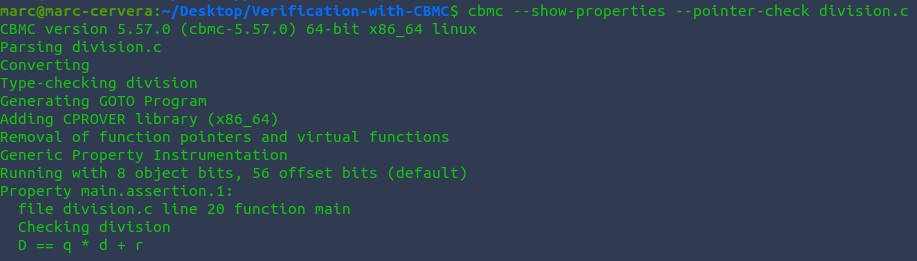
\includegraphics[scale = 0.7]{images/props.jpg}
    \caption{List of properties}
    \label{fig:props}
\end{figure}

\justify{The last step is to check the different \textit{asserts}. This will be performed by typing the following command in the CMD:\\}

\begin{lstlisting}
cmbc --unwind k division.c
\end{lstlisting}

\justify{After executing the above command with \textit{k = 301}, to perform 300 iterations, the \textit{assertion} works ok. So, the verification is successful, as it can be seen in the following picture.}

\begin{figure}[H]
    \centering
    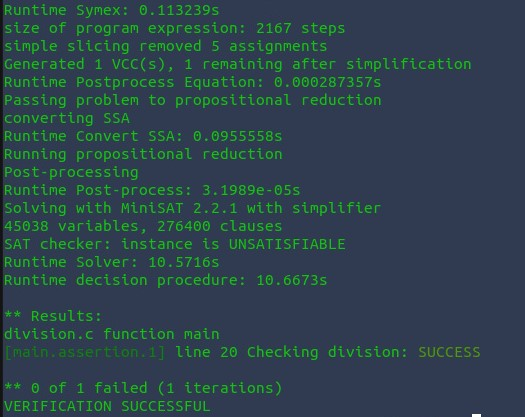
\includegraphics{images/ex1-succesful.jpg}
    \caption{Successful verification of the exercise 1 code.}
    \label{fig:success1}
\end{figure}

\subsubsection{Exercise 3:}
\textbf{Check for integer overflow bugs.\\}
\justify{To check for integer overflow bugs, the following command has to be executed in the CMD:\\}

\begin{lstlisting}
cbmc --trace --unwind k --signed-overflow-check division.c
\end{lstlisting}

\justify{After executing the above fixing the value of \textit{k} to 301, the algorithm cannot find any overflow bug, as can be seen in the following picture.}

\begin{figure}[H]
    \centering
    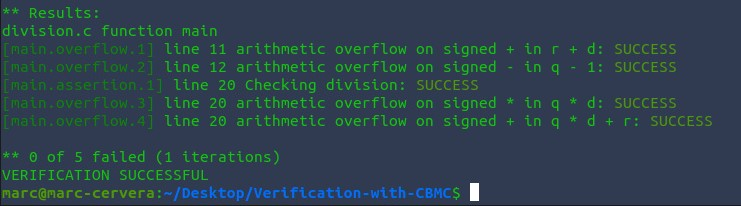
\includegraphics[scale = 0.7]{images/301arithmetic.jpg}
    \caption{Integer overflow bugs check performing 300 iterations.}
    \label{fig:300integerBug}
\end{figure}

\justify{To finish this exercise, it will proceed to check if fixing the value of \textit{k} to 1001, any bug can be found.}

\begin{figure}[H]
    \centering
    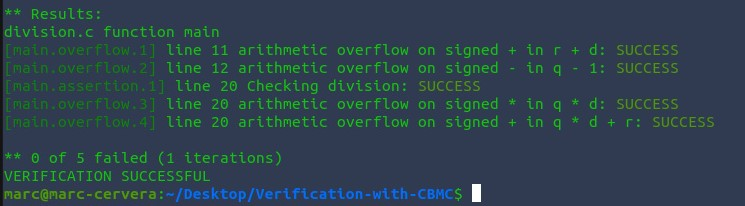
\includegraphics[scale = 0.7]{images/1001arithmetic.jpg}
    \caption{Integer overflow bugs check performing 1000 iterations.}
    \label{fig:1000integerBug}
\end{figure}

\justify{As it can be seen, neither with 1000 iterations, the algorithm can find any overflow bug.}

\section{Second problem}
\subsection{"simpleWhile.c" file}
\justify{Source code:}

\begin{lstlisting}
#define N 10
int main(){
    int numbers[N];
    int maxeven;
    int x = 0, i = 0;
    
    maxeven = 1;
    for(i = 0; i < N; i++){
        if(numbers[i] % 2 == 2){
            if(maxeven == 1 || maxeven < numbers[i]){
                maxeven = numbers[i];
            }
        }
    }
    if(maxeven != 1){
        // there are even numbers in the array,
        //so check that maxeven is the greatest one of them
    } else{
        // check that are NO even numbers in the array
    }
}
\end{lstlisting}

\subsubsection{Exercise 1:}
\textbf{Insert assertions at the end of the program for checking if there are even numbers in the array, then the maxeven is equal to the greatest even number.\\}
\justify{The first step, is to add the following code fragment to the source code file to be able to check that, in case that maxeven $\neq$ 1, the maxeven is the greatest number of all the even numbers of the array:\\}

\begin{lstlisting}
//...
if(maxeven != 1){
    for(i = 0; i < N; i++){
        __CPROVER_assert(numbers[i] <= maxeven, "The maxeven is >= to any numbers[i]");
    }
}
//...
\end{lstlisting}

\justify{The second part of this exerrcise is to check that if maxeven = 1, then there are no even numbers in the array. To check this property, the following code fragment has to be added:\\}

\begin{lstlisting}
/...
else{
    for(i = 0; i < N; i++){
        __CPROVER_assert(numbers[i] % 2 != 0, "Checking that all the numbers in numbers[i] are odd.");
    }
}
//...
\end{lstlisting}

\justify{Hence, the full source code file, after the modifications, looks like:}
\newpage

\begin{lstlisting}
#define N 10
int main(){
    int numbers[N];
    int maxeven;
    int x = 0, i = 0;
    
    maxeven = 1;
    for(i = 0; i < N; i++){
        if(numbers[i] % 2 == 2){
            if(maxeven == 1 || maxeven < numbers[i]){
                maxeven = numbers[i];
            }
        }
    }
    if(maxeven != 1){
        for(i = 0; i < N; i++){
            __CPROVER_assert(numbers[i] <= maxeven, "The maxeven is >= to any numbers[i]");
        }
        // there are even numbers in the array,
        //so check that maxeven is the greatest one of them
    } else{
        for(i = 0; i < N; i++){
            __CPROVER_assert(numbers[i] % 2 != 0, "Checking that all the numbers in numbers[i] are odd.");
        }
        // check that are NO even numbers in the array
    }
}
\end{lstlisting}

\justify{If the CBMC show properties command is executed, the following list of properties will be shown:\\}

\begin{figure}[H]
    \centering
    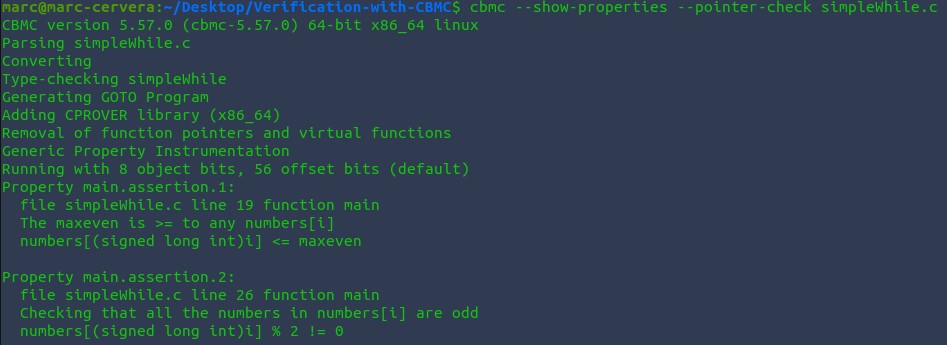
\includegraphics[scale = 0.7]{images/exercise2.jpg}
    \caption{Properties list of the second problem}
    \label{fig:propList2}
\end{figure}

\justify{After executing the CBMC verification, one of the \textit{assertions} that has been coded, fail. This is so obvious, because the content of the array is a binary decision. Or all the numbers are even or all the are odd, so one of the \textit{assertions} has to fail. Indeed, the evidences can be seen in the following picture:\\}

\begin{figure}[H]
    \centering
    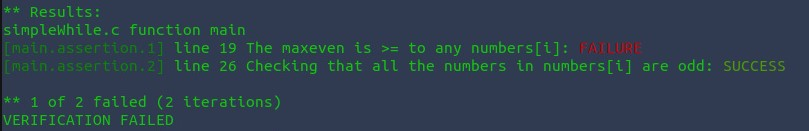
\includegraphics[scale = 0.8]{images/fail2.jpg}
    \caption{Results of the verification}
    \label{fig:failedVerification}
\end{figure}

\justify{To perform the verification the command used is:\\}

\begin{lstlisting}
cbmc simpleWhile.c
\end{lstlisting}

\subsubsection{Exercise 2:}
\textbf{Check that there are not "out of bounds errors" in the lines that operate with the array.}

\justify{To check if there are "out of bounds errors", the following command has to be executed in the CMD:\\}

\begin{lstlisting}
cbmc simpleWhile.c --bounds-check --pointer-check
\end{lstlisting}

\justify{In the following picture, can be seen that executing the above command, all the $\texttt{array\_bounds}$ pass the verification successfully.\\}

\begin{figure}[H]
    \centering
    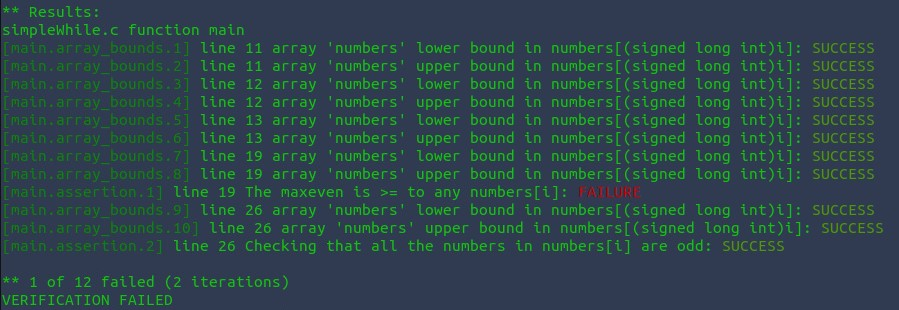
\includegraphics[scale = 0.7]{images/array_bounds.jpg}
    \caption{Array bounds verification}
    \label{fig:array_bounds}
\end{figure}

\justify{The global verification fails because of the already commented at the first exercise of this problem.}
\newpage

\section{Third problem}
\subsection{"sort.c" file}
\justify{Source code:}

\begin{lstlisting}
#include <stdint.h>
#define N 8

void sort(int8_t a[], int size){
    // write your favorite sorting algorithm
}

void checkSort(){
    int8_t array[N];
    int i;
    for (i = 0; i < N; ++i){
        // Assume numbers in array are integers in range [0, 16]
        __CPROVER__assume(array[i] >= 0 & array[i] <= 16);
    }
    
    sort(array, N);
    
    //write the assertions to check that the array is sorted
}
\end{lstlisting}

\subsubsection{Exercise 1:}
\textbf{Implement the sort function with your favorite sorting algorithm.}

\justify{The chosen sorting algorithm is the bubble sort algorithm. To know how works the algorithm this link has to be followed: \underline{\href{https://en.wikipedia.org/wiki/Bubble_sort}{Bubble sort}}.}
\justify{Once the algorithm is implemented, the sort function code looks like:\\}

\begin{lstlisting}
//...
void sort (int8_t a[], int size) {
	/*Bubble sort algorithm*/
	int i, j;
	for(i = 0; i < size - 1; i++){
		for(j = 0; j < size - i - 1; j++){
			if(a[j] > a[j + 1]){
				swap(&a[j], &a[j + 1]);
			}
		}
	}
}
//...
\end{lstlisting}

\subsubsection{Exercise 2:}
\textbf{Write assertions at the end of the checkSort function to verify if your sorting algorithm works as expected. Check with cbmc the function checkSort, but with four different values of N: $\{ \textbf{6, 8, 10, 12} \}$. Write down the computation time needed by cbmc to verify the program with these four different array sizes. Do you think that the computation time increases exponentially?}

\justify{Test for an array of 6 positions:}

\begin{figure}[H]
    \centering
    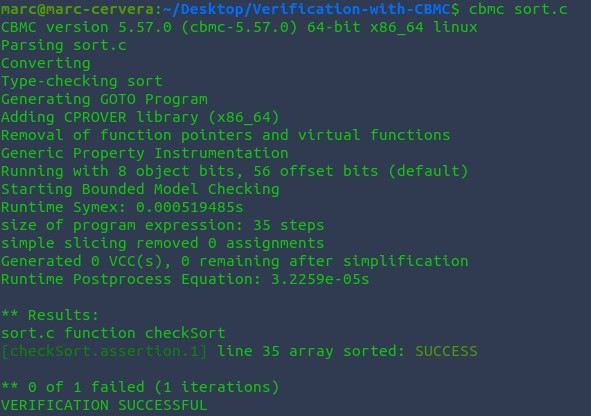
\includegraphics{images/testN6.jpg}
    \caption{Testing the sorting algorithm with N = 6}
    \label{fig:bubble6}
\end{figure}

\justify{Time $\longrightarrow$ 3.2259x10^{-5} seconds.}

\begin{figure}[H]
    \centering
    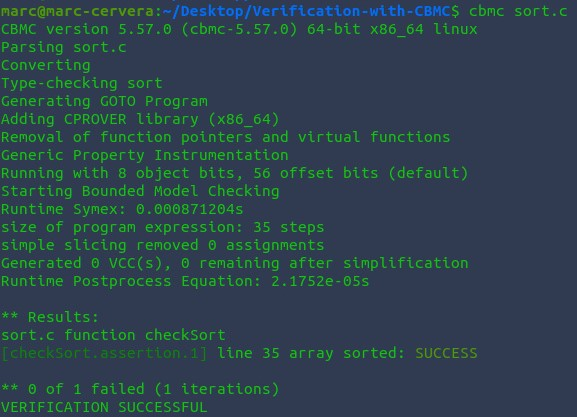
\includegraphics{images/testN8.jpg}
    \caption{Testing the sorting algorithm with N = 8}
    \label{fig:bubble8}
\end{figure}

\justify{Time $\longrightarrow$ 2.1752x10^{-5} seconds.}

\begin{figure}[H]
    \centering
    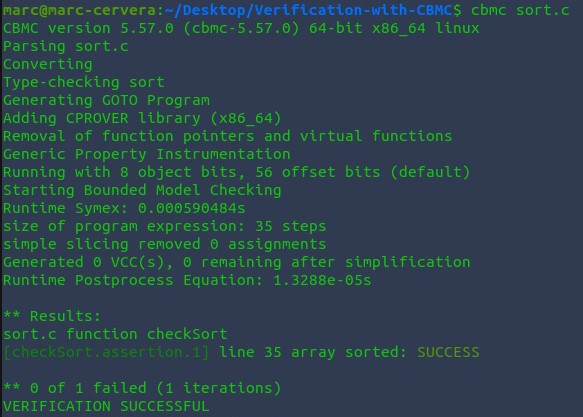
\includegraphics{images/testN10.jpg}
    \caption{Testing the sorting algorithm with N = 10}
    \label{fig:bubble10}
\end{figure}

\justify{Time $\longrightarrow$ 1.3288x10^{-5} seconds.}

\begin{figure}[H]
    \centering
    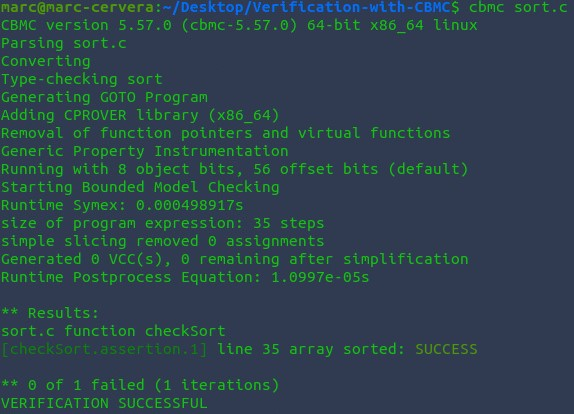
\includegraphics{images/testN12.jpg}
    \caption{Testing the sorting algorithm with N = 12}
    \label{fig:bubble12}
\end{figure}

\justify{Time $\longrightarrow$ 1.0997x10^{-5} seconds.}

\justify{To check if the time has en exponential order, the last step is to create a graphic with all the times.}

\begin{figure}[H]
    \centering
    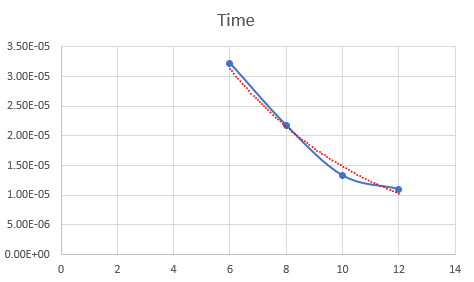
\includegraphics[scale = 0.7]{images/image_2022-06-14_135506513.png}
    \caption{Execution times with an exponential trend line}
    \label{fig:exptrend}
\end{figure}

\justify{As it can be seen, the exponential trend line does not fit very well. As it can be seen in the following picture the trend line that fits better is a polynomial trend line of third order:}

\begin{figure}[H]
    \centering
    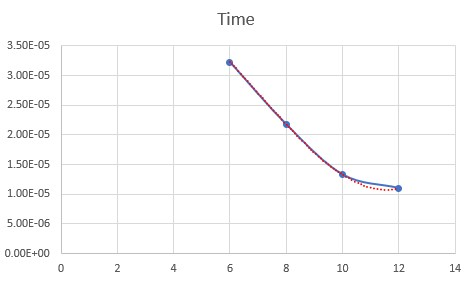
\includegraphics{images/poltrendline.jpg}
    \caption{Execution times with a polynomial trend line}
    \label{fig:poltrend}
\end{figure}

\end{document}
